\documentclass[a4paper, 14pt,russian]{extarticle}

\usepackage[russian]{babel}
\usepackage[T2A]{fontenc}
\usepackage[utf8]{inputenc}
%Соответствующий математический шрифт для Times new roman
\usepackage{newtxmath}
\usepackage{fontspec} 
%\usepackage{polyglossia}
%Times new roman
\defaultfontfeatures{Ligatures={TeX},Renderer=Basic} 
\setmainfont[Ligatures={TeX,Historic}]{Times New Roman}
\setmainfont{Times New Roman}
\setsansfont{Arial}
\setmonofont{Courier New}
\newfontfamily\cyrillicfont[Script=Cyrillic]{Times New Roman}
\newfontfamily\cyrillicfontsf[Script=Cyrillic]{Arial}
\newfontfamily\cyrillicfonttt[Script=Cyrillic]{Courier New}

%\setdefaultlanguage{russian}

%Геометрия
\usepackage{geometry}
\geometry{top=20mm}
\geometry{bottom=15mm}
\geometry{left=20mm}
\geometry{right=15mm}
\usepackage{setspace}
%Нормальные дроби через запятую
\usepackage{ncccomma}

\newcommand{\changefont}{%
	\fontsize{12}{11}\selectfont
}

%Заголовки
\usepackage{fancyhdr}
\pagestyle{fancy}
\fancyhf{}
%\renewcommand{\sectionmark}[1]{\markright{#1}}
\fancyhead[R]{\changefont \slshape \leftmark}
\fancyhead[L]{\changefont \slshape \rightmark}
%\newcommand{\ssubsection}[1]{\subsection*{#1}
%	\addcontentsline{toc}{subsection}{#1}
%	\markright{#1}{}}
\cfoot{\thepage}

%\полуторный интервал
\setstretch{1.15}
\setlength{\parindent}{1.25cm}

\usepackage{amsmath, amsfonts, mathtools}
\usepackage{physics}
\usepackage{indentfirst}
\usepackage{xcolor}
\usepackage{alltt}
\usepackage{graphicx}
\usepackage{wrapfig}
\usepackage{tikz}
\usetikzlibrary{calc}
\usetikzlibrary{shapes.geometric, shapes.misc, arrows}

\tikzstyle{startstop} = [rectangle, rounded corners, 
minimum width=3cm, 
minimum height=1cm,
text centered, 
draw=black]

\tikzstyle{io} = [trapezium, 
trapezium stretches=true, % A later addition
trapezium left angle=70, 
trapezium right angle=110, 
minimum width=3cm, 
minimum height=1cm, text centered, 
draw=black]

\tikzstyle{process} = [rectangle, 
minimum width=3cm, 
minimum height=1cm, 
text centered, 
text width=5cm, 
draw=black]

\tikzstyle{decision} = [diamond, 
minimum width=3cm, 
minimum height=1cm, 
text centered,
text width=3.5cm, 
draw=black]
\tikzstyle{arrow} = [thick,->,>=stealth]

\tikzstyle{startfor} = [chamfered rectangle, 
chamfered rectangle corners={north west, north east},
minimum width=3cm, 
minimum height=1cm, 
text centered, 
draw=black]

\tikzstyle{endfor} = [chamfered rectangle, 
chamfered rectangle corners={south west, south east},
minimum width=3cm, 
minimum height=1cm, 
text centered, 
draw=black]
\tikzstyle{arrow} = [thick,->,>=stealth]

%Настройка ссылок
\usepackage{hyperref}
%\usepackage{upgreek}
%\renewcommand{\beta}{\upbeta}
\hypersetup{
	colorlinks,
	citecolor=black,
	filecolor=black,
	linkcolor=black,
	urlcolor=black
}
\usepackage{caption}
\DeclareCaptionLabelSeparator{dot}{. }
\captionsetup{justification=centering,labelsep=dot}
\usepackage{titlesec}

%Формат заголовков
\titleformat{\section}{\bfseries\filcenter\Large}{\thesection}{1em}{}
\titleformat{\subsection}{\bfseries\filcenter\large}{\thesubsection}{1em}{}
\titleformat{\subsubsection}{\bfseries\filcenter\normalsize}{\thesubsubsection}{1em}{}

\usepackage{chngcntr}

%Включить в нумерацию картинок раздел
\counterwithin{figure}{section}

%Листинги кода и их стили
\usepackage{listings}
\usepackage{minted}
\lstdefinestyle{c++} {
	language=C++,
	breaklines=true,
	frame=single,
	numbers=left,
	basicstyle=\footnotesize\ttfamily,
	keywordstyle=\bfseries\color{green!40!black},
	commentstyle=\itshape\color{purple!40!black},
	identifierstyle=\color{blue},
	backgroundcolor=\color{gray!10!white},
}

\lstdefinestyle{python}{
	language=Python,
	breaklines=true,
	frame=single,
	numbers=left,
	keywordstyle=\bfseries\color{green!40!black},
	frame=lines,
	basicstyle=\footnotesize\rmfamily
}

\lstdefinestyle{cmd}{
	breaklines=true,
	frame=single,
	basicstyle=\footnotesize\ttfamily,
	frame=lines
	basicstyle=\footnotesize
}

\begin{document}
	
	\begin{titlepage}
	\newpage
	\begin{center}
		
\includegraphics[width=\textwidth]{png/tit.png}
		Институт информационных и вычислительных технологий \\
			Кафедра управления и интеллектуальных технологий
		\vspace{1.25cm}
	\end{center}
	
	\vspace{1.2em}
	
	\begin{center}
		%\textsc{\textbf{}}
		\begin{spacing}{1}
			{\Large Отчёт по лабораторной работе №2 \linebreak
			По дисциплине <<Управление в больших системах>> \\}
			\large{\bf<<Структурный анализ больших систем управления>>}
		\end{spacing}
	\end{center}
	
	\vspace{5em}
	

	\vspace{6em}
	
		\noindent Выполнил студент: Михайловский М.\,Ю. \\
		Группа: А-03-21 \\
		Вариант: 5\\
		Проверили: Новиков В.\,Н, Обычайко Д.\,C.
	
	
	\vspace{\fill}
	
	\begin{center}
		Москва 2024
	\end{center}
	
\end{titlepage}
	\pagenumbering{arabic}
	\setcounter{page}{2}
	\tableofcontents
	\newpage
	

	\section{Постановка задачи}
	
	Дана матрица смежности $A\in\mathbb{R}^{n\cross n}$, определяющая ориентированный граф системы с заданными в ней весами дуг: $G = (V, E)$.	Необходимо реализовать процедуру упорядочения вершин по уровням и нахождения минимальных путей в графе.	
	
	
	\setcounter{MaxMatrixCols}{20}
	\begin{equation}
		A = 
		\begin{bmatrix}
			0 & 0 & 0 & 0 & 0 & 0 & 0 & 0 & 2 & 0 & 0 & 0 & 0 & 0 & 0 & 0 & 0 \\
			0 & 0 & 0 & 0 & 0 & 0 & 0 & 0 & 0 & 0 & 0 & 0 & 0 & 0 & 0 & 0 & 2 \\
			0 & 0 & 0 & 6 & 4 & 0 & 5 & 0 & 0 & 0 & 3 & 0 & 0 & 0 & 0 & 0 & 0 \\
			0 & 0 & 0 & 0 & 0 & 0 & 0 & 0 & 2 & 0 & 0 & 0 & 0 & 0 & 0 & 0 & 0 \\
			0 & 0 & 0 & 3 & 0 & 4 & 0 & 0 & 0 & 0 & 0 & 0 & 0 & 0 & 0 & 0 & 0 \\
			0 & 0 & 0 & 0 & 0 & 0 & 0 & 0 & 0 & 0 & 0 & 3 & 0 & 0 & 0 & 0 & 0 \\
			2 & 0 & 0 & 2 & 0 & 0 & 0 & 0 & 5 & 0 & 0 & 0 & 0 & 0 & 0 & 0 & 0 \\
			0 & 0 & 0 & 0 & 0 & 0 & 0 & 0 & 0 & 0 & 0 & 0 & 0 & 2 & 0 & 0 & 0 \\
			0 & 0 & 0 & 0 & 0 & 0 & 0 & 0 & 0 & 0 & 0 & 0 & 0 & 0 & 0 & 3 & 0 \\
			0 & 0 & 0 & 0 & 0 & 0 & 0 & 0 & 0 & 0 & 0 & 0 & 0 & 0 & 1 & 0 & 0 \\
			3 & 4 & 0 & 0 & 0 & 0 & 0 & 0 & 0 & 0 & 0 & 0 & 0 & 0 & 0 & 0 & 0 \\
			0 & 0 & 0 & 0 & 0 & 0 & 0 & 0 & 0 & 0 & 0 & 0 & 0 & 0 & 0 & 2 & 0 \\
			0 & 0 & 0 & 0 & 0 & 0 & 0 & 0 & 0 & 0 & 0 & 0 & 0 & 0 & 2 & 0 & 0 \\
			0 & 0 & 0 & 0 & 0 & 0 & 0 & 0 & 0 & 0 & 0 & 0 & 0 & 0 & 2 & 0 & 0 \\
			0 & 0 & 0 & 0 & 0 & 0 & 0 & 0 & 0 & 0 & 0 & 0 & 0 & 0 & 0 & 0 & 0 \\
			0 & 0 & 0 & 0 & 0 & 0 & 0 & 0 & 0 & 3 & 0 & 0 & 3 & 0 & 0 & 0 & 0 \\
			0 & 0 & 0 & 0 & 0 & 0 & 0 & 2 & 0 & 0 & 0 & 0 & 0 & 0 & 0 & 0 & 0
		\end{bmatrix}
	\end{equation}
	
	Граф $G$, который задан такой матрицей смежности $A$ показан на рис. \ref{graph}. Как видно, граф является довольно сложным, и визуальный анализ системы при работе с таким графом будет затруднён, поскольку его структура весьма запутанная. 
	
	Для более простого анализа такой системы далее в работе будет проведено упорядочивание вершин.

	\begin{center}
		\begin{tikzpicture}[
				main/.style= {draw, circle},
				arr/.style= {font = {\footnotesize}}
			]
			\foreach \a in {1,2,...,17}{
				\node (\a) [main] at (\a*360/17: 3.75cm) {\a};
			}
			
			\draw [arrow, arr] (3) -- (7) node [midway, above] {5};
			\draw [arrow, arr] (7) to [out=90, in=135] node [above] {2} (4);
			\draw [arrow, arr] (3) -- (4) node [midway, above] {6};
			\draw [arrow, arr] (4) -- (9) node [midway, above] {2};
			\draw [arrow, arr] (7) to [out=180, in=140] node [midway, left] {5} (9);
			\draw [arrow, arr] (9) -- (16) node [midway, above] {2};
			\draw [arrow, arr] (16) -- (10) node [midway, above right] {3};
			\draw [arrow, arr] (10) to [out=-30, in=145] node [midway, below left] {1} (15);
			
			\draw [arrow, arr] (3) to [out=-120, in=75] node [midway, above] {3} (11);
			\draw [arrow, arr] (11) -- (2) node [midway, above] {4};
			\draw [arrow, arr] (2) to [out=0, in=45] node [midway, above right] {2} (17);
			\draw [arrow, arr] (17) -- (8) node [midway, above] {2};
			\draw [arrow, arr] (8) to [out=-45, in=150] node [midway, above] {2} (14);
			\draw [arrow, arr] (14) -- (15) node [midway, above left] {2};
			
			
			\draw [arrow, arr] (3) to [out=120, in=60] node [midway, above] {4} (5);
			\draw [arrow, arr] (5) -- (4) node [midway, above] {3};
			\draw [arrow, arr] (5) -- (6) node [midway, above] {3};
			\draw [arrow, arr] (6) -- (12) node [midway, above left] {3};
			\draw [arrow, arr] (12) -- (16) node [midway, above] {2};
			\draw [arrow, arr] (16) to [out=-60, in=-60] node [midway, above right=1cm] {3} (13);
			\draw [arrow, arr] (11) -- (1) node [midway, above] {3};
			\draw [arrow, arr] (7) -- (1) node [midway, above] {2};
			\draw [arrow, arr] (1) to [out=180, in=45] node [midway, above] {2} (9);
			\draw [arrow, arr] (13) to [out=-30, in=-90] node[midway, below left] {2} (15);
		\end{tikzpicture}
		\captionof{figure}{Граф данной системы}
		\label{graph}
	\end{center}

	\section{Подход к решению задачи}
	
	\subsection{Упорядочивание вершин}	
	
	Упорядочивание на $L+1$ уровней $N = \left\{N_0,\,N_1,\,\dots\,N_L\right\}$ проводится, исходя из множеств левых инциденций $i$-ых узлов: $G^{-1}(i)$ ($i=\overline{1,\,n}$), по принципу (\ref{levels}):
	\begin{equation}
		\begin{aligned}
			N_0 = &\left\{ i\,\mid\, G^{-1}(i) \varnothing \right\} \\
			N_1 = &\left\{ i\,\mid\, G^{-1}(i) \subset N_0 \right\} \\
			N_2 = &\left\{ i\,\mid\, G^{-1}(i) \subset \left(N_0\cup N_1\right) \right\} \\
			&\vdots \\
			N_L = &\left\{ i\,\mid\, G^{-1}(i) \subset \bigcup_{k=0}^{L-1} N_k \right\}
		\end{aligned}
		\label{levels}
	\end{equation}
	
	В результате упорядочивания легко построить граф этой же системы в виде, более наглядно представляющем структуру системы. 
	
	\subsection{Нахождение наименьшего пути}
	
	В данной работе реализован алгоритм, похожий на алгоритм Дейкстры, но учитывающий упорядоченную структуру графа. Всем вершинам, кроме начальной задаётся метка равная $\infty$. Начальной вершине задаётся метка, равная 0. Алгоритм начинает работу с $0$-ого уровня.
	\begin{enumerate}
		\item Рассматриваются все дуги инцидентные текущему уровню;
		\item Если для пары $(u, v)$ вершин соответствующих такой дуге $c(u) + c((u, v)) < c(v)$ ($c(u)$ - метка вершины $u$, $c((u, v))$ - цена дуги), то на вершину $v$ ставится метка равная этой сумме;
		\item Если текущий уровень $L-1$, то завершить алгоритм. Иначе перейти на следующий уровень. 
	\end{enumerate}
	
	\section{Реализованная программа}
	
	\subsection{Техническое описание}
	
	Программа реализована на \textit{Python 3.11.5} с модулями \textit{PyQt6, numpy, networkx, matplotlib}. Программа состоит из следующих основных модулей (листинг которых приведён в приложении):
	\begin{itemize}
		\item \textbf{main.py} -- Основной модуль, использующийся для запуска программы;
		\item \textbf{userInfo.py} -- модуль для получения и проверки введённых пользователям данных;
		\item \textbf{tableHandlers.py} -- модуль для работы с таблицей, в которой задаётся матрица смежности $A$;
		\item \textbf{GraphOptimizer.py} -- модуль для упорядочивания вершин графа и поиска минимальных путей;
		\item \textbf{GraphDrawer.py} -- модуль для построения визуализации упорядоченного графа;
		\item \textbf{my\_networkx.py} -- вспомогательный к \textbf{GraphDrawer.py} модуль, используемый для проставления весов на дугах, которые построены с кривизной;
		\item \textbf{main\_window.ui} -- разметка окна программы.
	\end{itemize}
	
	\subsection{Пример работы программы}
	
	При открытии программы появляется окно, представленное на рис. \ref{screen1}. Здесь можно ввести исходную матрицу $A$. 
	
	\begin{figure}[h]
		\centering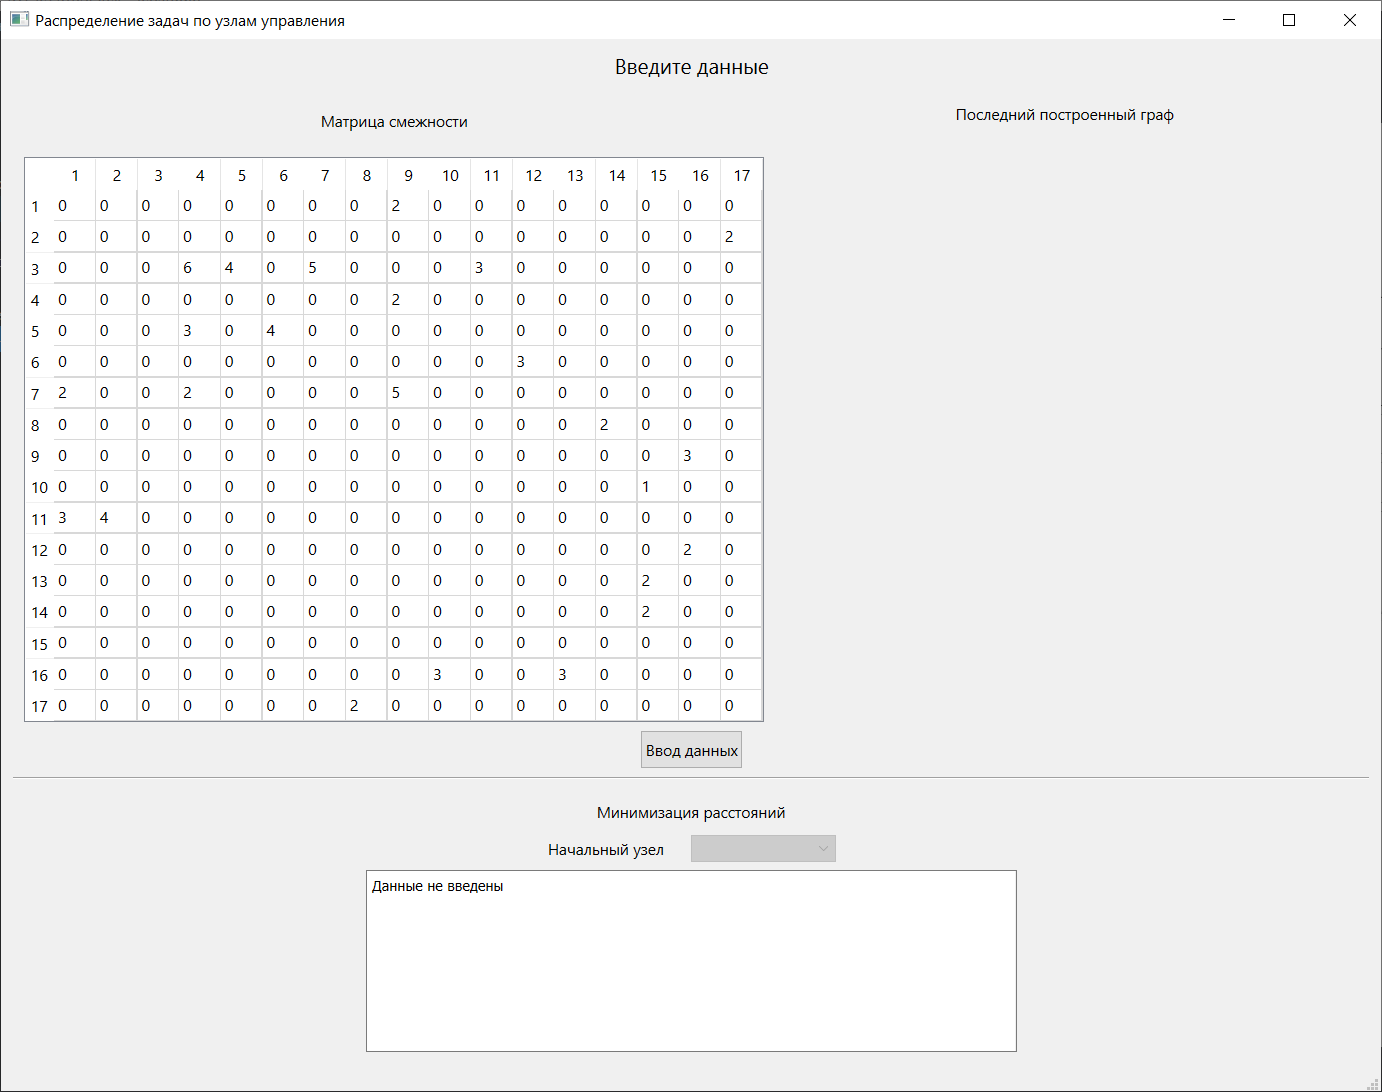
\includegraphics[width=.65\textwidth]{png/screen1.png}
		\caption{Основное окно программы}
		\label{screen1}
	\end{figure}
	
	После нажатия кнопки <<Ввод данных>> заполненная матрица $A$ считывается и строится упорядоченный граф, как на рис. \ref{screen2}.
	
	\begin{figure}[h]
		\centering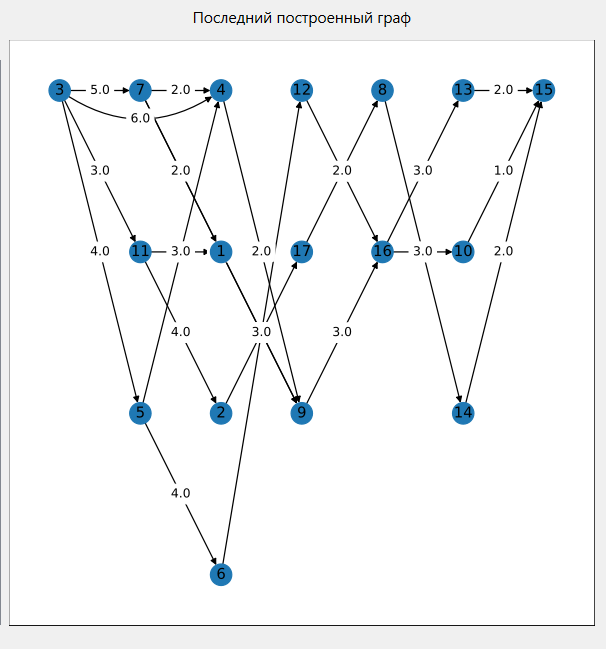
\includegraphics[width=.55\textwidth]{png/screen2.png}
		\caption{Построенный упорядоченный граф}
		\label{screen2}
	\end{figure}
	
	После этого в блоке снизу можно выбрать начальный узел для расчёта минимальных путей. Будут выведены списком только достижимые из выбранного начального узла вершины: рис. \ref{screen3}-\ref{screen4}.
	
	\noindent\begin{minipage}{0.45\textwidth}
		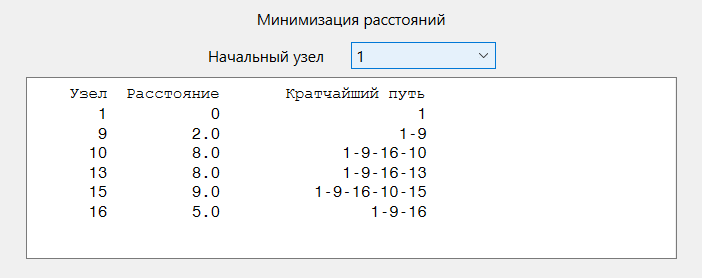
\includegraphics[width=\textwidth]{png/screen3.png}
		\captionof{figure}{Пример минимальных путей из узла 1}
		\label{screen3}
	\end{minipage}
	\begin{minipage}{0.45\textwidth}
		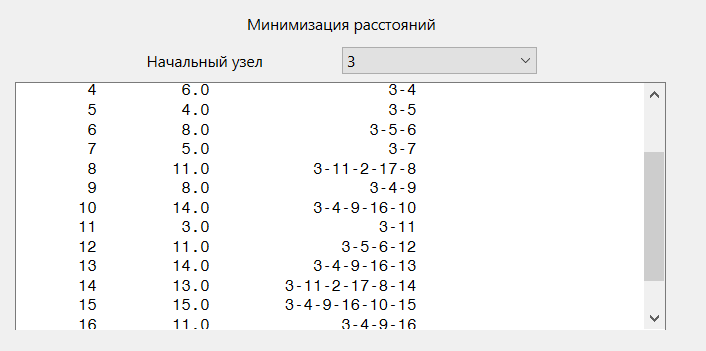
\includegraphics[width=\textwidth]{png/screen4.png}
		\captionof{figure}{Пример минимальных путей из узла 3}
		\label{screen4}
	\end{minipage}
	
	\newpage
	\section{Выводы}
	
	В данной работе была реализована программа для работы с ориентированными графами с заданными ценами дуг. В ней было реализовано две основные процедуры:
	\begin{itemize}
		\item Упорядочивание вершин введённого графа по уровням -- это позволяет представить граф в удобном для анализа структуры системы виде;
		\item Нахождение минимального пути между заданными вершинами.
	\end{itemize}
	
	\newpage 
	\appendix
	\titleformat{\section}{\normalfont\large\bfseries}{\centering Приложение \thesection. }{0pt}{\large\centering}
	\renewcommand{\thesection}{\Asbuk{section}}
	\section{Блок-схемы алгоритмов}
	
	\begin{center}
		\begin{tikzpicture}
			\node (start)[startstop] {Начало};
			\node (curLevel)[process, below=1.5cm] at (start) {Текущий уровень = 0};
			\draw [arrow] (start) -- (curLevel);
			
			\node (while) [decision, below=1.5cm] at (curLevel) {Распределили все вершины?};
			\draw [arrow] (curLevel) -- (while) node (aboveWhile) [midway] {};
			
			\node (end)[startstop, below right = 2.5cm] at (while) {Конец};
			\draw [arrow] (while) -| (end) node [midway, above] {Да};
			
			\node (raspr)[process, below=1.5cm] at (while.south) {Распределяем на текущий уровень вершины, в которые входят дуги из распределённых вершин};
			\draw [arrow] (while) -- (raspr) node[midway, right] {Нет};
			
			\node (newLevel) [process, below=1.5cm] at (raspr.south) {Текущий уровень += 1};
			\draw [arrow] (raspr) -- (newLevel);
			\draw [arrow] (newLevel.south) |- ++(-4cm, -1.5cm) |- (aboveWhile.center);
		\end{tikzpicture}
	\end{center}
	\captionof{figure}{Распределение по уровням}
	
	\begin{center}
		\begin{tikzpicture}
			\node (start)[startstop] {Начало};
			\node (curLevel)[process, below=1.5cm] at (start) {Текущий уровень = 0};
			\draw [arrow] (start) -- (curLevel);
			
			\node (while) [decision, below=1.5cm] at (curLevel) {Текущий уровень $< L$?};
			\draw [arrow] (curLevel) -- (while) node (aboveWhile) [midway] {};
			
			\node (end)[startstop, below right = 2.5cm] at (while) {Конец};
			\draw [arrow] (while) -| (end) node [midway, above] {Нет};
			
			\node (smotr)[process, below=1.5cm] at (while.south) {Смотрим правые инциденции $e=(u, v)$ вершин текущего уровня};
			\draw [arrow] (while) -- (smotr) node[midway, right] {Да};
			
			\node (metka)[process, below=1.5cm] at (smotr.south) {Присуждаем метку $c(v) = \min\left\{ c(v), c(u)+c(e)\right\}$};
			\draw [arrow] (smotr) -- (metka);
			
			\node (newLevel) [process, below=1.5cm] at (metka.south) {Текущий уровень += 1};
			\draw [arrow] (metka) -- (newLevel);
			\draw [arrow] (newLevel.south) |- ++(-4cm, -1.5cm) |- (aboveWhile.center);
		\end{tikzpicture}
	\end{center}
	\captionof{figure}{Нахождение минимальных путей}
	
	\newpage
	\section{Листинг программы}
	
	\captionof{lstlisting}{main.py}
	\label{main.py}
	\inputminted[frame=lines,fontsize=\footnotesize,breaklines=true,numbers=left]{python}{../main.py}	
	
	\captionof{lstlisting}{userInfo.py}
	\label{userInfo.py}
	\inputminted[frame=lines,fontsize=\footnotesize,breaklines=true,numbers=left]{python}{../userInfo.py}	
	
	\captionof{lstlisting}{tableHandlers.py}
	\label{tableHandlers.py}
	\inputminted[frame=lines,fontsize=\footnotesize,breaklines=true,numbers=left]{python}{../tableHandlers.py}	
	
	\captionof{lstlisting}{GraphOptimizer.py}
	\label{GraphOptimizer.py}
	\inputminted[frame=lines,fontsize=\footnotesize,breaklines=true,numbers=left]{python}{../GraphOptimizer.py}	
	
	\captionof{lstlisting}{GraphDrawer.py}
	\label{GraphDrawer.py}
	\inputminted[frame=lines,fontsize=\footnotesize,breaklines=true,numbers=left]{python}{../GraphDrawer.py}	
	
	\captionof{lstlisting}{my\_networkx.py}
	\label{my_networkx.py}
	\inputminted[frame=lines,fontsize=\footnotesize,breaklines=true,numbers=left]{python}{../my_networkx.py}	
	
	\captionof{lstlisting}{main\_window.ui}
	\label{main_window.ui}
	\inputminted[frame=lines,fontsize=\footnotesize,breaklines=true,numbers=left]{xml}{../main_window.ui}
	
\end{document}
